\documentclass[
a4paper,
%13pt,
fontsize=13pt
]{report}

\usepackage[T2A]{fontenc}
\usepackage[utf8]{inputenc}
\usepackage[russian]{babel}
\usepackage{setspace}
\usepackage[fontsize=14pt]{scrextend}
\usepackage[table,xcdraw]{xcolor}
%\usepackage[hscale=0.78,vscale=0.8]{geometry} % margins
\usepackage[
left=30mm,
right=10mm,
bottom=20mm,
top=15mm
]{geometry}

\usepackage{sectsty}
\chaptertitlefont{\LARGE}

%\titlespacing*{\chapter}{0pt}{3.5ex plus 1ex minus .2ex}{2.3ex plus .2ex}
\usepackage{titlesec}
\titleformat{\chapter}{\normalfont\LARGE\bfseries}{\thechapter}{1em}{}




\usepackage{amsmath} 
\usepackage{listings}
\usepackage{pdflscape}
\usepackage{graphicx}
\usepackage{subfig}
\usepackage[hidelinks]{hyperref}
%\usepackage[colorlinks = true, linkcolor=black, urlcolor=black]{hyperref}
\usepackage{amssymb}
\usepackage[numbers]{natbib}
\usepackage{enumerate}
%\usepackage{color}

\usepackage{verbatim}
\usepackage{minted}

%\renewcommand{\thefigure}{\arabic{section}.\arabic{figure}}
%\renewcommand{\thetable}{\arabic{section}.\arabic{table}}

\begin{document}
\onehalfspacing
\begin{titlepage}
  
  \begin{center}
    \textbf{% Министерство науки и высшего образования \\
      % Российской Федерации\\
      Федеральное государственное автономное образовательное
      учреждение высшего образования\\
      <<Российский университет дружбы народов имени Патриса Лумумбы>>}\\[5mm]
    Факультет физико-математических и естественных наук \\[2mm]
    Кафедра прикладной информатики и теории вероятностей

    \vfill

    
    
    \vfill

    Направление: 09.03.03 Прикладная информатика

    \vfill

    ОТЧЕТ

    \bigskip
    
    о прохождении учебной практики

    Научно-исследовательская работа
    
    (получение первичных навыков научно-исследовательской работы)

    \medskip
    
    Место прохождения практики: отдел технической поддержки
    пользователей (департамент технологических и информационных
    ресурсов) РУДН и научные центры института прикладной математики
    и телекоммуникаций
   
    Сроки прохождения: с «17» апреля 2023 г. по «17» июня 2023 г.
  \end{center}

\vfill

  \begin{minipage}{.45\textwidth}
    ФИО: Саргсян Арам Грачьяевич\\
    Курс, группа 3, НПИбд-02-20\\
    Студенческий билет № 1032201740 \\ \\
    Руководители практики: \\
    от РУДН к.ф.-м.н. Е.Г. Медведева \\ \\
    
    Научный руководитель: \\
    к.ф.-м.н., доц. А.В. Королькова \\ \\

    Руководитель от организации:\\
    д.т.н., проф. К.Е. Самуйлов
    
    % Выполнил: \\ [2mm]
    % студент группы НПИ-02-20\\[2mm]
    % \underline{\hspace{3cm}} Саргсян Арам Грачьяевич\\
    % (студенческий билет № 1032201740) \\[2mm] \\
    % ``\underline{\hspace{1cm}}''\underline{\hspace{3cm}}20\underline{\hspace{1cm}}г.
  \end{minipage}%
  \hfill
  
   
\vfill
Оценка \underline{\hspace{3cm}}

\centering
г. Москва

\
\centering
2023 г.
\end{titlepage}

%\newpage
\setcounter{page}{2}
\tableofcontents
\newpage
%\chapter*{Список используемых сокращений}
\addcontentsline{toc}{chapter}{Список используемых сокращений}

\mbox{}

RED --- Random Early Detection

TCP --- Transmission control protocol

NS  --- Network Simulator

NAM --- Network animator



\chapter*{Введение}
\addcontentsline{toc}{chapter}{Введение}

%\textcolor{red}{Данная работа посвящена ...}

% Беспроводные коммуникационные сети сегодня широко используются во
% многих приложениях, начиная от прямой связи между электронными
% устройствами и заканчивая интеллектуальными транспортными
% системами. Среди наиболее популярных беспроводных технологий --- Vanet
% SUMO (Simulation of Urban MObility) - это программное обеспечение для
% моделирования дорожного движения с открытым исходным кодом,
% разработанное Немецким аэрокосмическим центром (DLR). Она моделирует
% поведение транспортных средств, пешеходов и общественного транспорта в
% городских районах и имитирует влияние различных сценариев на дорожное
% движение.



Согласно программе учебной практики по направлению 09.03.03
«Прикладная информатика», целями практики являются:
\begin{itemize}
\item формирование навыков использования современных научных методов
  для решения научных и практических задач;
\item формирование универсальных, общепрофессиональных и
  профессиональных компетенций в соответствии с ОС ВО РУДН;
\item формирование навыков проведения исследовательской работы;
\item формирование навыков работы с источниками данных;
\item знакомство с принципами функционирования и изучение методов разработки и анализа моделей функционирования сложных систем, их фрагментов и отдельных элементов;
\item применение методов для анализа и расчёта показателей функционирования сложных систем, их фрагментов и отдельных элементов.
\end{itemize}

Также опредены задачи практики:
\begin{itemize}
\item изучение специфики функционирования и соответствующих  методов анализа сложных систем;
\item формирование навыков решения конкретных научно-практических задач самостоятельно или в научном коллективе; 
\item формирование навыков проведения исследовательской работы и получении научных и прикладных результатов;
\item изучение принципов и методов построения моделей сложных систем (в том числе технических систем, сетей и систем телекоммуникаций);
\item изучение принципов и методов анализа поведения параметров моделей сложных систем (в том числе программных и технических систем, сетей и систем телекоммуникаций, и т. п.);
\item приобретение практических навыков в области изучения научной литературы и (или) научно-исследовательских проектов в соответсвии с будущим    профилем профессиональной области.
\end{itemize}


Для достижении вышеупомянутых целей и задач в рамках учебной практики по теме "Моделирования алгоритма управления очередями RED в средстве моделирования NS-2" мною было выполнено следующее:
\begin{itemize}
\item рассмотрены основные методы имитационного, аналитического и натурного моделирования сетей;
\item исследована специфика моделирования различных сетей c помощью программы NS-2;
\item проведен сравнительный анализ результатов имитационнойого моделирования сети(графики размера TCP-окна, длины очереди и средней взвешанной очереди) при различных модификациях алгоритма RED, разных пороговых значений и видов TCP-окна. 
\end{itemize}

%\newpage
\chapter{Методы и материалы}
\section{NS-2}
NS-2(Network simaulator 2) — это программное средство моделирования сетей, использующиеся 
для исследования и анализа поведения компьютерных сетей. 
Запуск симуляции в данной среде позволяет анализировать различные протоколы и алгоритмы сетевой связи. 
NS-2 разработан на языке программирования С++ и TCL, что обеспечивает гибкость и расширяемость средства моделирования. 
NS-2 содержит библиотеку классов, представляют различные элементы сети, такие как узлы, маршрутизаторы, каналы связи и протоколы передачы данных. Для создания модели сети определяются характеристики и параметры каждого элемента сети: пропускная способность каналов, задержки, вероятность потери пакетов и другие. После завершения симуляции NS-2 предоставляет мощные инструменты анализа результатов, включая возможность визуализации данных посредством программы NAM(Network animator), статический анализ и сравнение экспериментов, что позволяет изучать и оценивать производительность различных протоколов и алгоритмов в различных сценариях сети~\cite{The2011,Floyd1997}.

\section{Mininet}
Mininet — это симулятор сетевых топологий на основе виртуаилизации, который позволяет моделировать и изучать поведение сетей в контролируемой среде, основанный на использовании виртуальных машин и пространств имен Linux для создания изолированных сетевых узлов. Моделирование сетевых топологией с помощью Mininet позволяет исследовать различные сетевые протоколые, маршрутизацию, управление трафиком и т. д. Возможности моделирования с помощью Mininet включают создание виртуальных сетевых узлов, конфигурирование топологий(связь между узлами, настраивать IP-адреса, маршрутизацию), имитировать различные условия сети, такие как задержки, потери пакетов и пропускную способность, интеграция с контроллерами для исследования новых протоколов и алгоритмов.

\section{Cisco Packet Tracer}
Packet Tracer — это программное средство, предоставляемое компанией Cisco Systems, позволяющей смоделировать, конфигурировать и отлаживать сетевые сценарии, широко используемое в области сетевых технологий. Данное программное обеспечение предоставляет виртуальную среду, которое позволяет создавать сетевые топологии и настраивать устройства Cisco: маршрутизаторы, коммутаторы, и т д. Графический интерфейс позволяет соединять устройства, устанавливать параметры соединений и задавать настройки протоколов. Cisco Packet Tracer позволяет имитировать передачу данных в сети. Пользователи могут выполнять различные тесты связи, проводить диагностику и мониторинг сетевых устройств, а также создавать и анализировать журналы событий.

\section{GNS-3}
GNS-3 — это программное средство моделирования сетей, позволяющий создавать виртуальные сети, состоящие из реальных или виртуальных устройств, и анализировать их поведение. GNS-3 разработан на языке программирования Python и основан на эмуляторе динамических узлов Dynamips, который позволяет запускать реальные образы операционных систем. В отличие от Packet Tracer, GNS-3 позволяет смоделировать не только устройства Cisco, но и другие устройства, как Juniper, Palo Alto и другие, что позволяет смоделировать различные типы сетей, включая центры обработки данных и облачные инфраструктуры. Одной из главных особенностей GNS-3 является интеграция с виртуальными машинами, что расширяет возможности моделирования. Появляется возможность создавать сетевые сценарии, в которых виртуальные машины выполняют реальные функции, такие как серверы, клиенты, точки доступа Wi-Fi и т. д. Это позволяет проводить натурное моделирование и получить более реалистичные результаты в рамках виртуальной среды.



Эта команда должна работать (см. рис.~\ref{fig:1.1}).


\begin{figure}[!h]
  \centering
  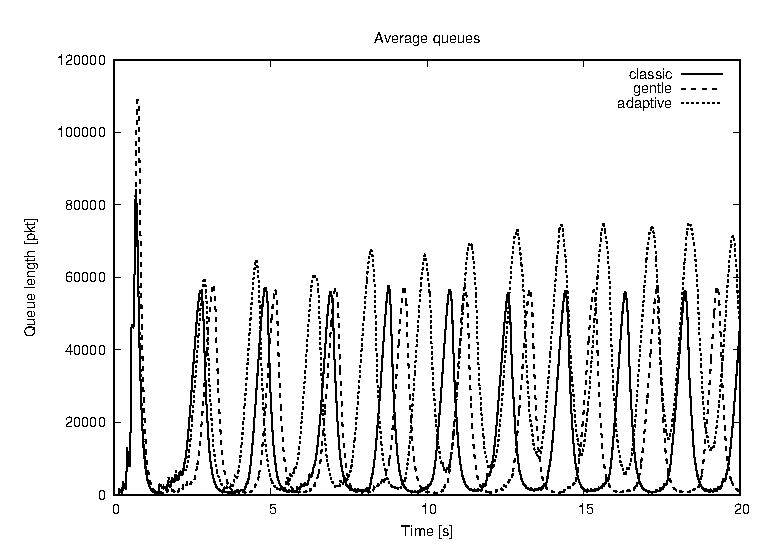
\includegraphics[width=0.9\linewidth]{image/av_queues_3types.eps}
  \caption{3 types of RED}
  \label{fig:1.1}
\end{figure}



\section{SUMO-модель движения транспорта для города Абиджан, коммуны Абобо}


Реализация модели VANET будет сделана для города Абиджан, а точнее для
коммуны Абобо.  Первым шагом будет загрузка xml-файла через карты с
сайта (\url{https://www.openstreetmap.org/.})  Вторым шагом будет
преобразование загруженного файла в xml-формат с помощью команды:
\begin{verbatim}
    netconvert --osm-files filename.osm -o filename.net.xml filename.net.xml
\end{verbatim}

На третьем шаге мы должны использовать файл в нашей папке sumo, мы скопируем
его и поместим в наш проект. Для этого воспользуемся командой:
\begin{verbatim}
    cd /home/directory/sumo-x.x/data/typemap
\end{verbatim}

Последний шаг перед компиляцией будет выполнен с помощью следующей команды
\begin{minted}[linenos,tabsize=2,breaklines]{bash}
    polyconvert --osm-files filename.osm --net-file filename.net.xml, --type-file osmPolyconvert.typ.xml -o filename.poly.xml
    python /home/directory/sumo-x.x/tools/randomtrips.py -n fileName.net.xml -r, fileName.rou.xml -e 50 -l
\end{minted}

Запуск программы (рис.~\ref{fig:1.3}):
\begin{verbatim}
    sumo-gui nomdufichier.sumo.cfg`
\end{verbatim}

\begin{figure}[!h]
  \centering
  \includegraphics[width=0.9\linewidth]{image/08.PNG}
  \caption{Фрагмент SUMO-модели движения транспорта для города Абиджан, коммуны Абобо}
  \label{fig:1.3}
\end{figure}





\chapter{RED}

\section{Classic RED}


Random Early Detection (RED) — это механизм предотвращения перегрузки
на шлюзе. Он основан на общих принципах, полезен для управления
средним размером очереди в сети, где не доверяют взаимодействию между
протоколами передачи данных. В отличие от Droptail, который работает
таким образом, что когда очередь заполняется, новые пакеты,
поступающие в очередь, начинают теряться, алгоритм RED учитывает
потоки трафика в сети и стремится предоставить равную пропускную
способность для каждого соединения, что позволяет избежать перегрузки
сети и улучшить качество обслуживания. В оригинальном RED
маршрутизатор вычисляет усредненный по времени средний размер очереди
с использованием фильтра нижних частот (экспоненциально взвешенное
скользящее среднее) или сглаживания по длине выборки очередей, средний
размер очереди сравнивается с двумя пороговыми значениями: минимальным
порогом и максимальным. Когда средний размер очереди меньше
минимального порога, пакеты не отбрасываются, когда средний размер
очереди превышает максимальный порог, отбрасывается все поступающие
пакеты. Если размер средней очереди находится между минимальным и
максимальным порогом, пакеты отбрасываются с вероятностью $p$, которая
линейно увеличивается до тех пор, пока средняя очередь не достигнет
максимального порога. Подробно алгоритм описан в~\cite{RED1,RED2}.
 
Вероятность $p_{b}$ маркировки на отбрасывание пакетов представляет
собой функцию, линейно зависящую от $\hat{q}$ (средневзвешенное
скользящее среднее), минимального $q_{\min}$ и максимального
$q_{\max}$ пороговых значений и параметра $p_{\max}$, определяющего
часть отбрасываемых пакетов при достижении средним размером очереди
значения $q_{\max}$ и вычисляется следующим образом(\ref{red}):
\begin{equation}
\label{red}
p_{b} = \begin{cases}
        0, &  \ 0 < \hat{q} \leqslant q_{\min},
        \\
        \frac{\hat{q} - q_{\min}}{q_{\max} - q_{\min}} p_{\max}, & \ q_{\min} < \hat{q} \leqslant q_{\max}, 
        \\
        1, &  \ \hat{q} > q_{\max}.
\end{cases}                                     
\end{equation}

График функции вероятности потери пакета в зависимости от среднего
размера очереди представлен на рис.~\ref{fig:2.1}.

\begin{figure}[!h]
  \centering
  \includegraphics[width=0.7\linewidth]{image/RED.png}
  \caption{Классический RED}
  \label{fig:2.1}
\end{figure}


В NS-2 файлы, связанные с RED, прописаны в каталоге
\verb|ns-2.35/queue|, там представлены также другие реализации
очередей (среди них DropTail, BLUE и т.д.). Следует уделить внимание
двум файлам: \verb|red.cc| (исходники), и \verb|red.h| (заголовочный
файл). Вероятность отбрасывания пакета прописана в функции
double \begin{verbatim} REDQueue::calculate_p_ne файла red.cc. \end{verbatim}


\section{GRED} 

GRED (Gentle Random Early Detection, мягкое/аккуратное произвольное
раннее обнаружение)~--- алгоритм активного управления очередью,
является расширением RED.  Стандартный алгоритм увеличивает
вероятность отбрасывания с 0.05 до 0.5, когда средняя длина очереди
увеличивается от минимального до максимального порогового значения, но
при превышении максимального порога вероятность возрастает напрямую с
0.5 до 2.  Этот внезапный скачок нормализуется модификацией Gentle
RED, который расширяет RED тем, что добавляет дополнительное
максимальное пороговое значние, которое равно $2q_{\max}$, тем самым
<<сглаживая>> кривую~\cite{GRED}. Для реализации модификации в NS-2
при описании очереди нужно задать переменную \verb|set gentle_ true|.

Вероятность сброса определяется следующим образом (\ref{gred}):

\begin{equation}
\label{gred}
p_{b} =\begin{cases}
        0, &  \  0 < \hat{q} \leqslant q_{\min}, 
        \\
        \frac{\hat{q} - q_{\min}}{q_{\max} - q_{\min}} p_{\max}, & \ q_{\min} \leqslant \hat{q} < q_{\max}, 
        \\
        \frac{\hat{q} - q_{\min}}{q_{\max}}(1-p_{\max}) - p_{\max}, & \ q_{\max} \leqslant \hat{q} < 2q_{\max}, 
        \\
        1, &  \ \hat{q} \geqslant  q_{\max}.
\end{cases}
\end{equation}

График функции вероятности потери пакета в зависимости от среднего
размера очереди выглядит следующим образом (рис.~\ref{fig:2.2}):

\begin{figure}[!h]
  \centering
  \includegraphics[width=0.7\linewidth]{image/GentleRED.jpg}
  \caption{Gentle RED}
  \label{fig:2.2}
\end{figure}

\section{WRED}

WRED (Weighted random early detection --- взвешенное произвольное раннее
обнаружение)~--- это алгоритм активного управления очередью, является
расширением RED~\cite{WRED}.

Взвешенный алгоритм произвольного раннего обнаружения предоставляет
различные уровни обслуживания пакетов в зависимости от вероятности их
отбрасывания и обеспечивает избирательную установку параметров
механизма RED на основании типа трафика (рис.~\ref{fig:2.3}).

\begin{figure}[!h]
  \centering
  \includegraphics[width=0.7\linewidth]{image/wred.png}
  \caption{Weighted RED}
  \label{fig:2.3}
\end{figure}

Алгоритм WRED работает с единой очередью пакетов, для которой, как и в
RED, по формуле рассчитывается экспоненциально взвешенное скользящее
среднее. Для каждого типа трафика задаются собственные параметры
(пороговые значения, максимальный уровень сброса) и вычисляется
вероятность сброса.

Например, очереди могут иметь более низкие пороговые значения для
более низких приоритетов пакета. Это приведет к отбрасыванию пакетов с
низким приоритетом, а следовательно, к защите пакетов с более высоким
приоритетом в той же очереди.

\section{NLRED}

Nonlinear RED~--- это модификация классического алгоритма RED, в
отличие от которого использует нелинейную функцию для определения
вероятности отбрасывания пакетов, что позволяет более гибко
регулировать процесс управления перегрузками, учитывая различные
характеристики трафика и динамику
сети~\cite{NLRED1,NLRED2}. Вероятность $p_{b}$ маркировки на
отбрасывание пакетов вычисляется следующим способом (\ref{nlred}):

\begin{equation}
\label{nlred}
p_{b} = \begin{cases}
        0, &  \ 0 < \hat{q} \leqslant q_{\min},
        \\
        1, &  \ \hat{q} > q_{\max},
        \\
        \frac{\hat{q} - q_{\min}}{q_{\max} - q_{\min}} {2.5p^{2}_{\max}}, & \ q_{\min} < \hat{q} \leqslant q_{\max}.
\end{cases}
\end{equation}

График функции вероятности потери пакета в зависимости от среднего
размера очереди представлен на  рис.~\ref{fig:2.4}.

\begin{figure}[!h]
  \centering
  \includegraphics[width=0.7\linewidth]{image/NonLinearRED.png}
  \caption{NonLinear RED}
  \label{fig:2.4}
\end{figure}

По умолчанию NLRED не реализован в NS-2. Для её добавления я проделал следующие шаги:

\begin{enumerate}
\item Установил к себе на машину патч \verb|NLRED.patch| от Mohit
  P. Tahiliani для версии 2.34, совместимой также для версии 2.35.
\item Отредактировал файл, заменив везде номер версии на 2.35 и
  переместил в каталог \verb|ns-allinone|.
\item В терминале запустил команду \verb|patch -p1 < NLRED.patch|, а
  затем запустил \verb|./install|.
\item В настройке очереди сети указал значение переменной \verb|nonlinear 2|.
\end{enumerate}
 
\section{ARED и RARED}

В алгоритме Adaptive RED (ARED) функция сброса модифицируется
посредством изменения по принципу AIMD, заключающейся в том, что
увеличение некоторой величины производится путём сложения с некоторым
параметром, у уменьшение~--- путём умножения на
параметр~\cite{RARED}. Для её реализации в NS-2 необходимо указать в
настройке очереди \verb|set adaptive 2|.

Алгоритм ARED функционирует следующим образом (\ref{ad1}),
(\ref{ad2}). Для каждого интервала \verb|interval| (параметр) в
секундах, если $\hat{q}$ больше целевой (желаемой) $\hat{q_t}$ и
$p_{\max} \leqslant 0,5$, то $p_{\max}$ увеличивается на некоторую
величину $\alpha$; в противном случае, если $\hat{q}$ меньше целевой
$\hat{q_t}$ и $p_{\max}\geqslant 0,01$, то $p_{\max}$ уменьшается в
$\beta$ раз:

\begin{equation}
\label{ad1}
p_{\max} = \left\{
  \begin{aligned}
    & p_{\max}+\alpha, \ \hat{q}>\hat{q_{t}}, \ p_{\max} \leqslant 0,5, \\
    & \beta p_{\max}, \ \hat{q}<\hat{q_{t}}, \ p_{\max} \geqslant 0,01, 
  \end{aligned}
\right.
\end{equation}

\begin{equation}
\label{ad2}
q_{\min}+0,4(q_{\max}-q_{\min}) < \hat{q_t} < q_{\min}+0,6\left(q_{\max}-q_{\min}\right).
\end{equation}

Основные особенности: 
\begin{itemize}
\item автоматическая установка минимального порога $q_{\min}$. Он
  устанавливается в зависимости от пропускной способности канала $C$ и
  задержки целевой очереди;
\item автоматическая установка максимального порога $q_{\max}$. Он
  устанавливается в зависимости от значения месяца;
\item автоматическая настройка $w_{q}$. Он устанавливается в
  зависимости от пропускной способности канала $C$;
\item адаптивная настройка $p_{\max}$. Он адаптирован в соответствии с
  текущей средней длиной очереди.
\end{itemize}

Алгоритм Refined ARED (\ref{rf1}), (\ref{rf2}) является модификацией
ARED и предлагает более активно изменять вероятность сброса $p_{\max}$,
чтобы иметь возможность быстрой адаптации к изменяющейся
экспоненциально взвешенной скользящей средней длине очереди $\hat{q}$:

\begin{equation}
\label{rf1}
p_{b} = \left\{
  \begin{aligned}
& p_{\max}+\alpha, \quad  \hat{q}>\hat{q_{t}}, \quad p_{\max} \leqslant 0,5, \\
& \beta p_{\max}, \quad \hat{q}\leqslant\hat{q_{t}}, \quad p_{\max} \geqslant 0,5,
  \end{aligned}
\right.
\end{equation}

\begin{equation}
\label{rf2}
\left\{
  \begin{aligned}
    & q_{\min}+0,48\left(q_{\max}-q_{\min}\right) < \hat{q_t} < q_{\min}+0,52\left(q_{\max}-q_{\min}\right), \\
    & \alpha=\left(0,25\frac{\hat{q}-\hat{q_t}}{\hat{q_t}} \right)p_{\max}, \\ 
    & \beta=1-\left(0,17\frac{\hat{q}-\hat{q_t}}{\hat{q_t}-q_{\min}}\right).
  \end{aligned}
\right.
\end{equation}


По умолчанию Refined ARED не реализован в NS-2. Для его добавления я
проделал следующие шаги:

\begin{enumerate}
\item Установил к себе на машину патч \verb|Re-ARED.patch| от Mohit
  P. Tahiliani для версии 2.34, совместимой также для версии 2.35.
\item Отредактировал файл, заменим везде номер версии на 2.35 и переместил в каталог \verb|ns-allinone|.
\item В терминале запустил команду patch \verb|-p1 < Re_ARED.patch|, а затем  \verb|./install|.
\item В настройке очереди сети указал значение переменной \verb|adaptive 1| и
  для RARED дополнительно \verb|refined adaptive 2|.
\end{enumerate}















\chapter{Результаты}

Мною была написана программа, реализующую натурную модель с 
базовой топологией с двумя хостами и одним коммутатором для реализации
программы.
 
Полная реализация программы приведена в разделе \textbf{Приложения},
для вывода графиков была использована программа GNUPLOT.

Смоделировал сеть три раза с указанными параметрами. В первом случае добавили задержку в 100 мс на обоих хостах, во втором случае 50мс, в третем случае 100мс с отклонением в 10мс и запустив gnuplot-скрипт, я получил следующий график(рис.~\ref{fig:3.1}).

\begin{figure}[!ht]
  \centering
  \includegraphics[width=0.6\linewidth]{image/pings.eps}
  \caption{Измерение задержек при разных условиях}
  \label{fig:3.1}
\end{figure}

Как мы видим из графика, наименьшие задержки имеет сеть с задержкой в 50 мс, при указании отклонения в 10мс задержки возрастают в несколько раз.


На коммутаторе s1 указал дисциплину очереди red со следующими параметрами: минимальный порог сброса в 30000 байтов, максимальный в 60000 байтов.
Смоделировал сеть и с помощью iperf3 получил графики окна перегрузки, пропускной способности и количества переданных байтов. Изменил дисциплину очереди c red на ared. Вывел соответствующие графики также и для этой модификации (рис.~\ref{fig:3.2}, \ref{fig:3.3}, \ref{fig:3.4}, \ref{fig:3.5}, \ref{fig:3.6}, \ref{fig:3.7}).

\begin{figure}[!ht]
  \centering
  \includegraphics[width=0.6\linewidth]{image/red/cwnd_red.pdf}
  \caption{Окно перегрузки при использовании red}
  \label{fig:3.2}
\end{figure}

\begin{figure}[!ht]
  \centering
  \includegraphics[width=0.6\linewidth]{image/ared/cwnd_ared.pdf}
  \caption{Окно перегрузки при использовании ared}
  \label{fig:3.3}
\end{figure}

Как мы видим, при классическом алгоритме размер TCP окна перегрузки значительно меньше. 


\begin{figure}[!ht]
  \centering
  \includegraphics[width=0.6\linewidth]{image/red/throughput_red.pdf}
  \caption{Пропускная способность при использовании red}
  \label{fig:3.4}
\end{figure}

\begin{figure}[!ht]
  \centering
  \includegraphics[width=0.6\linewidth]{image/ared/throughput_ared.pdf}
  \caption{Пропускная способность при использовании ared}
  \label{fig:3.5}
\end{figure}

Сравнивая графики пропусеной способности, мы видим, что  adaptive red имеет в среднем немного большую пропускную способность. 

\begin{figure}[!ht]
  \centering
  \includegraphics[width=0.6\linewidth]{image/red/bytes_red.pdf}
  \caption{Количество переданных данных при использовании red}
  \label{fig:3.6}
\end{figure}

\begin{figure}[!ht]
  \centering
  \includegraphics[width=0.6\linewidth]{image/ared/bytes_ared.pdf}
  \caption{Количество переданных данных при использовании ared}
  \label{fig:3.7}
\end{figure}

При ARED также имеем большее количество переданных байтов. 




\chapter*{Заключение}
\addcontentsline{toc}{chapter}{Заключение}

% Мобильные сети Ad Hoc (MANETs) и автомобильные сети (VANETs) --- это два
% типа беспроводных сетей, которые обеспечивают мобильную и автономную
% связь между устройствами. Протокол IEEE 802.11p специально разработан
% для VANET, обеспечивая высокоскоростную связь с низкой задержкой для
% приложений безопасности дорожного движения и автономного вождения.
% Zigbee, с другой стороны, является беспроводной технологией с низким
% энергопотреблением и низкой скоростью передачи данных, используемой в
% основном в беспроводных сенсорных сетях (WSN) для таких приложений,
% как домашняя автоматизация, управление энергопотреблением и т.д.  В
% целом, MANET и VANET предназначены для обеспечения мобильной и
% автономной связи между устройствами, в то время как беспроводные
% технологии, такие как IEEE 802.11p и Zigbee, специально разработаны
% для удовлетворения специфических требований приложений, для которых
% они используются. Выбор правильной технологии для конкретного
% приложения будет зависеть от конкретных коммуникационных требований
% этого приложения.


За период практики были достигнуты цели и решены поставленные задачи,
определенные в программе учебной практики направления подготовки
02.04.02 «Фундаментальная информатика и информационные технологии»
(см. введение отчета по практике).

В ходе прохождении практики: 
\begin{itemize}
\item работал с научной терминологией области исследований, научился
  собирать и обобщать информацию по теме исследований (УК-1, УК-7, ПК-1);
\item с помощью научного руководителя определил круг задач для
  достижения поставленных передо мной целей практики (УК-2);
\item планировал выполнение работ в рамках задания по практике, а также
  консультации с научным руководителем, что позволило своевременно в
  срок провести самостоятельное изучение научной и учебной литературы,
  выполнить базовое исследование в рамках темы; заполнен дневник
  прохождения практики, отражающий выполнение заданий, используемые
  ресурсы и результаты (УК-3, УК-5, УК-6);
\item работал с источниками информации на русском, французском и
  английском языках (УК-4);
\item для решения основной задачи по имитационному моделированию VANET
  использовал современные средства моделирования NS-3, SUMO (ОПК-1,
  ОПК-3, ПК-1).
\end{itemize}


Таким образом, в рамках учебной практики мною было выполнено:
\begin{itemize}
\item кратко рассмотрены технология VANET, средства имитационного моделирования SUMO и NS3;
\item установлено программное обеспечение: SUMO и NS-3 под ОС Linux;
\item реализован пример моделирования движения транспорта для города Абиджан, коммуны Абобо в SUMO;
\item запущен пример модели VANET в NS-3.
\end{itemize}

\renewcommand{\bibname}{Список литературы}
\cleardoublepage
\phantomsection
\addcontentsline{toc}{chapter}{Список литературы}
\bibliography{bib}

\bibliographystyle{ugost2008l} 
% \bibliographystyle{plain} 
% \bibliographystyle{gost2008l} 

\appendix

\chapter*{Приложения}
\addcontentsline{toc}{chapter}{Приложения}

Ссылка на репозиторий: 
\url{https://github.com/agsargsyan/study_2022-2023_practice}

\section*{Программа симуляции топологии с red}

\begin{minted}[linenos,tabsize=2,breaklines]{bash}
-#!/usr/bin/env python

"""
Simple experiment.
Output: ping.dat
"""
from mininet.net import Mininet
from mininet.node import Controller
from mininet.cli import CLI

from mininet.log import setLogLevel, info
import time

def emptyNet():

   "Create an empty network and add nodes to it."

   net = Mininet( controller=Controller, waitConnected=True )

   info( '*** Adding controller\n' )
   net.addController( 'c0' )

   info( '*** Adding hosts\n' )
   h1 = net.addHost( 'h1', ip='10.0.0.1' )
   h2 = net.addHost( 'h2', ip='10.0.0.2' )

   info( '*** Adding switch\n' )
   s1 = net.addSwitch( 's1' )

   info( '*** Creating links\n' )
   net.addLink( h1, s1, bw = 10 )
   net.addLink( h2, s1, bw = 10 )

   info( '*** Starting network\n')
   net.start()

   info( '*** Set red options\n')
   s1.cmdPrint( 'tc qdisc add dev s1-eth1 root handle 1: red limit 1000000  max 30000 min 60000 burst 80 avpkt 1000 bandwidth 10Mbit ' )
   
   #для ARED
   #s1.cmdPrint( 'tc qdisc add dev s1-eth1 root handle 1: red limit 1000000  max 30000 min 60000 burst 80 avpkt 1000 bandwidth 10Mbit adaptive' )	


   info('*** Traffic generation\n')
   h2.cmdPrint('iperf3 -s -D -1 ')
   time.sleep(21) # Wait 21 seconds
   h1.cmdPrint('iperf3 -c', h2.IP(),'-J > iperf_result.json')

   info( '*** Ping\n')
   h1.cmdPrint( 'ping -c 10', h2.IP(), '| grep "time=" | awk \'{print $5, $7}\' | sed -e \'s/time=//g\' -e\'s/icmp_seq=//g\' > ping.dat' )

   info( '*** Stopping network' )
   net.stop()

if __name__ == '__main__':
    setLogLevel( 'info' )
    emptyNet()
    
% \end{verbatim}
\end{minted}


\section*{Makefile}

\begin{minted}[linenos,tabsize=2,breaklines]{bash}
all: ping.dat ping.pdf plot

ping.dat:
	sudo python lab_netem_i.py
	sudo chown mininet:mininet ping.dat

ping.pdf: ping.dat
	  ./ping_plot

plot: iperf_result.json
	plot_iperf.sh iperf_result.json

clean:
	-rm -f *.dat *.pdf *.json *.csv
	-rm -rf results
\end{minted}

\section*{}

\begin{minted}[linenos,tabsize=2,breaklines]{bash}

#!/usr/bin/gnuplot --persist

set terminal png crop
set output 'ping.pdf'
set xlabel "Sequence number"
set ylabel "Delay (ms)"
set grid
plot "ping.dat" with lines

\end{minted}









\appendix
 %\newpage

\end{document}
